\documentclass[12pt,a4paper]{article}
\usepackage[latin2]{inputenc}
\usepackage{graphicx}
\usepackage{ulem}
\usepackage{amsmath}
\usepackage[margin=0.5in]{geometry}
\usepackage[T1]{fontenc}
\usepackage[ampersand]{easylist}
\usepackage[english]{babel}
\usepackage{scrextend}
\usepackage{subfig}
\usepackage{float}
\usepackage{stackengine}
\usepackage{listings}
\usepackage{epstopdf}
%\usepackage[demo]{graphicx}
%\usepackage{caption}
%\usepackage{subcaption}
%\usepackage[utf8]{inputenc}
\begin{document}

%%%%%%%%%%%%%%%%%%%%%%%%%%%%%%%%%%%%%%%%%%%%%%%%%%%%%%%%%%%%%%%%%%%%%%%%%%%%%%%%
% Document Setup

\pagenumbering{arabic}

%%%%%%%%%%%%%%%%%%%%%%%%%%%%%%%%%%%%%%%%%%%%%%%%%%%%%%%%%%%%%%%%%%%%%%%%%%%%%%%%
% Title block - Page 0

% Cover page. Clearly indicate the names of the team members.

\author{
  Singireddi, Sanjana\\
  \texttt{sanjana9@stanford.edu}\\
  \texttt{SUID:xxxxxxxx}
  \and
  Lenius, Samuel\\
  \texttt{lenius@stanford.com}\\
  \texttt{SUID:06091240}
}

\title{2016 EE214B Design Project - Part I}

\maketitle

\pagebreak

%%%%%%%%%%%%%%%%%%%%%%%%%%%%%%%%%%%%%%%%%%%%%%%%%%%%%%%%%%%%%%%%%%%%%%%%%%%%%%%%
% Bias Calculations - Page 2

% Bias point calculations for part I (a). Include a comparison with SPICE
% results from part (b) by providing a table that states the percentage
% deviations in the calculated voltages, g m and rpi.

\section{Bias Calculations}
\par

Bias calculations go here.\par

%\begin{figure}[H]
%	\footnotesize
%	\stackunder[5pt]{\includegraphics[width=0.5\textwidth]{cmv_vs_vz.png}}{}
%	\hfill
%	\stackunder[5pt]{\includegraphics[width=0.5\textwidth]{vz_vs_vy.png}}{}
%\end{figure}

\pagebreak

%%%%%%%%%%%%%%%%%%%%%%%%%%%%%%%%%%%%%%%%%%%%%%%%%%%%%%%%%%%%%%%%%%%%%%%%%%%%%%%%
% Calculations c-f, pages 3-6

\section{Calculation of Key Design Parameters}

\textbf{Choice of L}

\begin{itemize}
\item All devices used in current source have a minimum length of 2$\mu$m.
\item All other devices in the amplifier have minimum length of 1$\mu$m. 
Minimum length is used as f$_{t }$ is inversely proportional to L.
\item All devices in bias generator circuit have length $>$=2$\mu$m.
\end{itemize}


\textbf{Bias Generator circuit}

\begin{itemize}
\item Constant gm reference based design is used as bias circuit to 
reduce mismatch errors.
\item Transconductance of bias device (mn300) depends only on R2 and m ( 
m is the ratio of MN300/MN400). Therefore gm can be set precisely.
\item Start-up circuit is used to force the circuit to the desired 
operating point.
\end{itemize}


\textbf{Approximations for hand calculations}

For simpler hand calculations, following approximations are used.

\newcounter{numberedCntBB}
\begin{enumerate}
\item $Cdb=Csb=0.35 Cgs$
\item $Cgs=(\frac{2}{3})WLCox+Cov'W$
\item $Cgd=Cov'W$
\item $gmb=0.2gm$
\setcounter{numberedCntBB}{\theenumi}
\end{enumerate}


\textbf{Stage4}

\begin{itemize}
	\item As per the spec, common mode output voltage (vout) has to be within -0.15v to 0.15v. Since the body is connected to vss, MN10 experiences back gate effect and the threshold voltage is given by:
	\begin{equation}
	\begin{split}
		Vt=Vt_0+ \gamma(\sqrt{2\phi f+V_{sb}}- \sqrt{2}\phi f\\
		Vt_0=0.5V , \gamma=0.6 , 2\phi f=0.8
	\end{split}
	\end{equation}


	\item Stage 4 is a source follower which has a gain given by
	\begin{equation}
		A4=\frac{gm_{10}}{gm_{10}+gmb_{10}+(\frac{1}{R_L})}
	\end{equation}
	\item Gain of stage4 (A4) $<$1 due to back gate effect and the output load. 
	\item To achieve gain closer to 1 (0.6 - 0.7), it is important to size and bias MN10 such that ($gm_{10}+ gmb_{10}) >> (1/R_L)$. 
	\item Transconductance of and drain current of $MN_{10}$ is given by 
	\begin{equation}
		gm_{10}= \mu nCox(\frac{W}{L})vov_{10}
	\end{equation}
	\begin{equation}
		Id_{10}=0.5\mu nCox(\frac{W_{10}}{L_{10}})vov_{10}^2 (1+\lambda (Vdd-Vout))
	\end{equation}
	\item $MN_9$ (bias device for source follower) is sized such that $Id_{10}+ I_{R_L}= Id_9$ and the common mode output voltage does not fall out of range. This device is chosen to be of smaller size to reduce loading on Vout node. 
	\begin{equation}
		\tau_{OUTPUT} = (R_L || \frac{1}{1.2gm_{10}})(C_L+Csb_{10}+Cgd_9+Cdb_9)
	\end{equation}
	\item Cgs10 is assumed to be very small due to boot-strapping.
\end{itemize}


\textbf{Stage 3}

\begin{itemize}
	\item Loading at node Vy increases with the increase in gain of stage 3 due to the miller effect. Hence gain of stage3 is kept low and is fixed at sqrt(2) to compensate for the gain lost in stage 4. Gain of stage3 (CS amplifier with diode connected load):
	\begin{equation}
		|A3|=\frac{gm7}{gm8}=\frac{Vov8}{Vov7}=\frac{Vdd-Vz-abs(Vtp)}{Vy-Vss-Vtn}=\sqrt{2}
	\end{equation}

	\item Choice of Vz from above (stage4) determines Vy.	
	\item Minimum device sizes (W=2$\mu$m, L=1$\mu$m) are used for both MN7 and MP8 to reduce loading on Vy and Vz.
	\begin{equation}
		Id_7=Id_8=0.5\mu nCox(\frac{W_7}{L_7})vov_7^{2} (1+\lambda(Vz-Vss))
	\end{equation}
	\begin{equation}
		\tau_Z=(\frac{1}{gm_8})(Cgs_8+Cdb_8+Cgd_{10}+Cgd_7(1+\frac{1}{|A3|})+Cdb_7)
	\end{equation}
\end{itemize}


\textbf{Stage 2}

\begin{itemize}
	\item Vy from stage Z above determines the required ratio of R3 and R4.
	\begin{equation}
		(\frac{R4}{R3})=\frac{Vss}{Vy}-1
	\end{equation}

	\item Gain of stage Y (Cascode amplifier) is set to 3.
	\begin{equation}
		|A2|=gm4(R3 || R4)
	\end{equation}
	\item $Vov_4$ and $W_{4}$ are optimized to reduce $\tau_X$.
\end{itemize}


%\begin{figure}[H]
%\centering
%\includegraphics[width=10.63cm,height=7.99cm]{tau_x_y_vs_mp4.png}
%\end{figure}


\begin{itemize}
	\item MN6 is sized such that current through MN6 is same as the current through MP4 and MP5. 
	\begin{equation}
		Id4=Id5=Id6=0.5\mu pCox(\frac{W4}{L4})(Vdd-Vx-abs(Vtp))^{2} (1+\lambda (Vdd-Vw)
	\end{equation}
	\item Current through R3 and R4
	\begin{equation}
		I_{R3}+I_{R4}=Vss/(R3+R4)
	\end{equation}
	\begin{equation}
		\tau_Y=(R3 || R4)(Cgs_7+Cgd_7 (1+|A3|)+Cgd_6+Cdb_6+Cgd_5+Cdb_5)
	\end{equation}
\end{itemize}


\textbf{Stage 1}

\begin{itemize}
	\item $Vov_4$ from stage 2 sets $V_X$ which in turn sets the ratio of R1 and R2.
	\begin{equation}
		Vov_4=Vdd-Vx-|Vtp|
	\end{equation}
	\begin{equation}
		(\frac{R1}{R2})=\frac{Vdd}{Vx}-1
	\end{equation}
	\item Gain of stage 1 (Common gate amplifier) is set to 10000.
	\begin{equation}
		|A1|=(R1 || R2)
	\end{equation}
	\item MN1 and MP3 are sized such that Id1 = Id3.
	\item MN2 is sized to reduce $\tau_{IIN}$ node.  $\tau_{IIN}$ is inversely proportional to $gm_2$.
	\begin{equation}
		\tau_{IIN}=(\frac{1}{gm2})(Cin+Cgd_1+Cdb_1+Cgs_2+Csb_2)
	\end{equation}
	\begin{equation}
		\tau_{X}=(R1 || R2)(Cgd_2+Cdb_2+Cgd_3+Cdb_3+Cgs_4+Cgd_4)
	\end{equation}
\end{itemize}



%\begin{figure}[h]
%\centering
%\includegraphics[width=10.63cm,height=7.99cm]{tau_i_x_vs_mn2.png}
%\end{figure}


\begin{itemize}
	\item Current through MN1, MN2 and MP3
	\begin{equation}
		Id_{1,2,3}=0.5\mu pCox(\frac{W_3}{L_3})(Vdd-VbiasP-|Vtp|)^{2} (1+\lambda (Vdd-Vx))
	\end{equation}
	\item Current through R1 and R2
	\begin{equation}
		I_{R1}+I_{R2}=Vdd/(R1+R2)
	\end{equation}
\end{itemize}

\textbf{Vovn, Vovp}

\begin{itemize}
	\item Vovn and Vovp are chosen to achieve a reasonable balance between gain, Tau total and Power, and our choice was educated by the gm/Id technology plots.
\end{itemize}
\textbf{Total Design Performance}
\begin{equation}
	|A_{TOTAL}|=A1* A2* A3* A4
\end{equation}
\begin{equation}
	\tau_{TOTAL}=\tau_{IIN}+\tau_X+\tau_Y+\tau_Z+\tau_{OUTPUT}
\end{equation}
\begin{equation}
	Power=(Vdd-Vss)(Id_1+Id_4+Id_7+Id_{10})+(\frac{Vdd^{2}}{R1+R2})+(\frac{Vss^{2}}{R3+R4})
\end{equation}

\begin{table}[h]
\centering
\begin{tabular}{|l|l|l|l|l|}
\hline
\textbf{Bias Generator} & Hand calc & Spice & \%Error & Reason for error \\
\hline
$V_{BiasN}$ & -1.300V &  -1.279V &  -1.6\% &  Startup circuit bias \\
\hline
$V_{BiasP}$ & 1.300V &  1.319V & 1.5\%  &  Startup circuit bias \\
\hline
  &   &   &   &   \\
\hline
\textbf{Stage1} & Hand calc & Spice & \%Error & Reason for error \\
\hline
$Id_1$ & 18.3$\mu$A  &  20.9$\mu$A &  14.2\% &  Bias generator error \\
\hline
Vx & 1.300V  & 1.275V  & -1.9\%  &   \\
\hline
$A_X$ & 10k$\Omega$  & 9.86k$\Omega$  & -1.4\%  & Finite $MN_1$ and $MP_3$ output resistance  \\
\hline
$gm_2$ &  210$\mu$S & 268$\mu$S  & 27.6\%  & Bias generator error  \\
\hline
$\tau_{IN} $ & 1.11ns  &   &   &   \\
\hline
$\tau_X $ & 420ps  &   &   &   \\
\hline
  &   &   &   &   \\
\hline
\textbf{Stage2} & Hand calc & Spice & \%Error & Reason for error \\
\hline
$Id_4$ &  36.75$\mu$A & 43.5$\mu$A & 18.4\%  &   \\
\hline
$V_W$ & 1.496V & 1.450V  & -3.2\%  &   \\
\hline
$V_Y$ & -1.550V  & -1.418V  &  -8.5\% & Imbalance between $MP_4$ and $MN_6$ current \\
\hline
$gm_4$ & 105$\mu$S  &  120$\mu$S & 14.3\%  & Error in $V_Y$ \\
\hline
$A_Y$ & -3.0  & -3.25  & 8.3\%  & Error estimating $gm_4$  \\
\hline
$\tau_Y$ & 306ps  &   &   &   \\
\hline
  &   &   &   &   \\
\hline
\textbf{Stage3} & Hand calc & Spice & \%Error & Reason for error \\
\hline
$Id_7$ & 10.25$\mu$A  & 22.9$\mu$A  & 123\%  & Error in $V_Y$ plus finite output resistance  \\
\hline
$V_Z$ & 1.364 & 1.102V  & -19.2\%  & Error in $V_Y$   \\
\hline
$gm_7$ & 45$\mu$S  & 79$\mu$S  & 75.5\%  &  Error in $Id_7$ \\
\hline
$gm_8$ & 31.2$\mu$S & 51$\mu$S   &  63.5\% &  Error in $Id_7$  \\
\hline
$A_Z$ & 1.414  & 1.440  & 1.8\%  &  The benefit of ratiometric design \\
\hline
$\tau_Z$ & 1.92ns  &   &   &  Error in estimating $gm_{8}$ \\
\hline
  &   &   &   &   \\
\hline
\textbf{Stage4} & Hand calc & Spice & \%Error & Reason for error \\
\hline
$Id_{10}$ & 2.96$\mu$A  &  30.43$\mu$A &  928\% & $MN_{10}$'s large width is a big error amplifier  \\
\hline
$V_{OUT}$ & 0.299 & -0.117V  &  -139\% &   \\
\hline
$Vt_{10}$ & 0.999  & 1.034V  &  3.5\% &   \\
\hline
$gm_{10}$ & 91.1$\mu$S   &  327$\mu$S  & 258\%  &   \\
\hline
$gmb_{10}$ & 13.0$\mu$S  &  55.1$\mu$S  & 323\%  &   \\
\hline
$A_{OUT}$ & 0.71 & 0.75  & 5.6\%  &   \\
\hline
$\tau_{OUT}$ & 1.63ns  &   &   & Error in estimating $gm_{10}$  \\

\hline
Total Power &  578$\mu$W & 1.065mW  & 84\%  & Not accounting for bias gen  \\
\hline
Total Gain & 30.04k$\Omega$  & 34.66k$\Omega$   &  15.5\% & Error in estimating gm  \\
\hline
\end{tabular}
\end{table}

\pagebreak
page
\pagebreak

%%%%%%%%%%%%%%%%%%%%%%%%%%%%%%%%%%%%%%%%%%%%%%%%%%%%%%%%%%%%%%%%%%%%%%%%%%%%%%%%
% Bode Diagrams - Page 7 & 8

% Bode plot and pz outputs for parts I (g) and (h). Be sure to include proper
% annotations, and comparisons to hand calculated values.

\section{Bode Plots and PZ Outputs - Part I(g,h)}

{\centering
	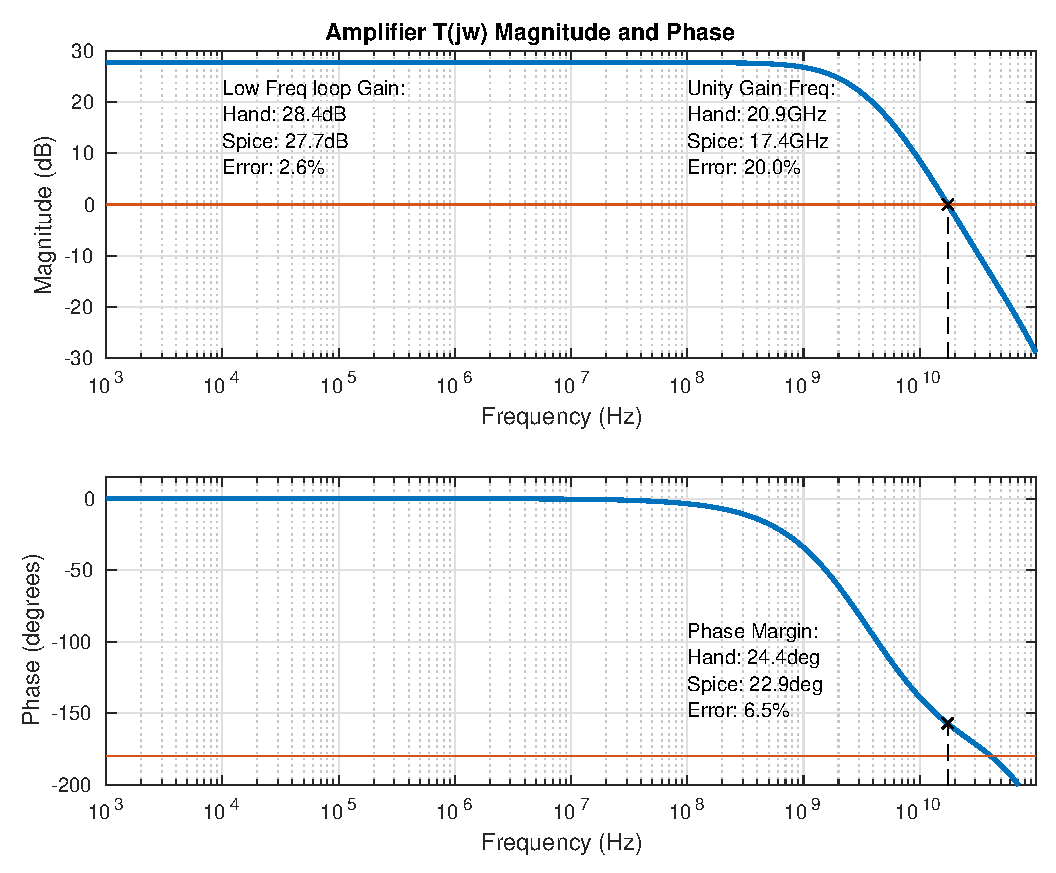
\includegraphics[width=0.8\textwidth]{plots/part_g.eps}
\par}

\pagebreak

{\centering
	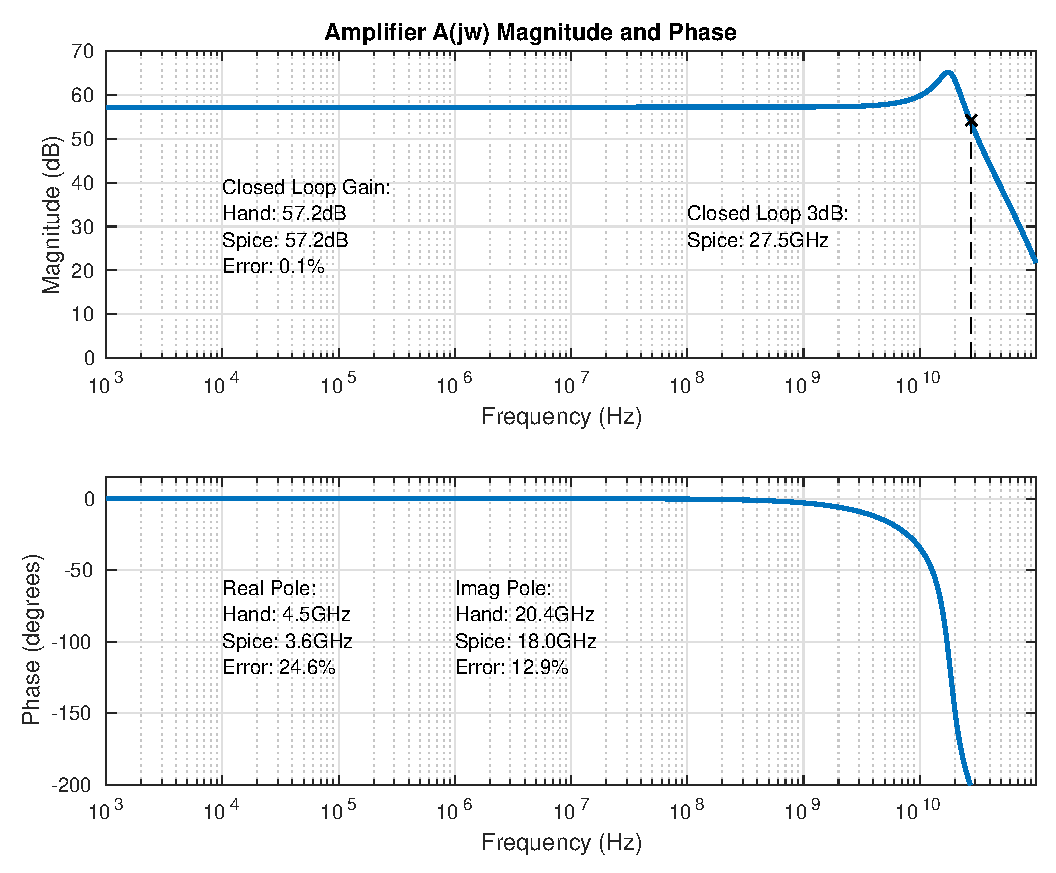
\includegraphics[width=0.8\textwidth]{plots/part_h.eps}
\par}

\begin{verbatim}
 ***************************************************
    ******   pole/zero analysis
    input =  0:is          output = v(vo)
    poles (rad/sec)                 poles ( hertz)
    real            imag            real            imag            
    -33.1562m       0.              -5.27698m       0.              
    -22.9305g       113.319g        -3.64950g       18.0353g        
    -22.9305g       -113.319g       -3.64950g       -18.0353g       
    -473.782g       0.              -75.4048g       0.              
    -1.12800t       0.              -179.526g       0.              
    -1.18039t       0.              -187.865g       0.              

    zeros (rad/sec)                 zeros ( hertz)
    real            imag            real            imag            
    0.              0.              0.              0.              
    -1.10418t       0.              -175.736g       0.   

\end{verbatim}

\pagebreak

%%%%%%%%%%%%%%%%%%%%%%%%%%%%%%%%%%%%%%%%%%%%%%%%%%%%%%%%%%%%%%%%%%%%%%%%%%%%%%%%
% Calculations for part I (i). - Page 9

\section{Calculations for Part I(i)}

% part i
% The capacitor Cf can be used to introduce a feedback zero. Estimate the value
% of Cf that yields a maximally flat response. What is the expected closed-loop
% bandwidth of the circuit?

%f_o = 1.7443184E+10;
%w_o = f_o * 2 * pi;
%w_z = w_o / sqrt(2);
%w_z = w_o / (sqrt(2) - (pole.vi.w + pole.vx.w) / w_o);
%c_z = 1 / (w_z * r_f);

%c_in_z = c_in + c_z;
%cl_3db_w = sqrt((1+k) / (r_in * c_in_z * r_x * c_x));
%cl_3db_f = cl_3db_w / (2 * pi);
A feedback capacitor can be used to introduce a zero into the feedback loop in
order to push the higher frequency pole out and flatten the response of the
closed loop amplifier. The optimally flat response of the amplifier occurs when Q = $\sqrt{2}$. Hence:

\begin{equation}
  \omega_0 = 1.09e11 rad/s
\end{equation}

\begin{equation}
  \omega_Z = \frac{\omega_{0}}{\sqrt{2} - \frac{\omega_{P1} + \omega_{P2}}{\omega_{0}}}
\end{equation}

\begin{equation}
  C_F = \frac{1}{\omega_Z R_F} = 57fF
\end{equation}

From this, the new closed loop bandwidth can be calculated as such:

\begin{equation}
  C_{in,C_F} = C_{in} + C_F
\end{equation}

\begin{equation}
  k = \frac{R_{in} * Q1_{gm} * R_x * A_{V3}}{R_F}
\end{equation}

\begin{equation}
  BW_{CL,C_F} = \frac{\sqrt{1 + k}}{2 \pi R_{in} C_{in} R_x C_x} = 19.2Ghz
\end{equation}

\pagebreak


%%%%%%%%%%%%%%%%%%%%%%%%%%%%%%%%%%%%%%%%%%%%%%%%%%%%%%%%%%%%%%%%%%%%%%%%%%%%%%%%
% Bode Diagrams - Page 10 & 11

% Bode plots and pz outputs for part I (j). Be sure to include proper
% annotations, and comparisons to hand calculated values.

\section{Bode Plots and PZ Outputs - Part I(j)}

{\centering
	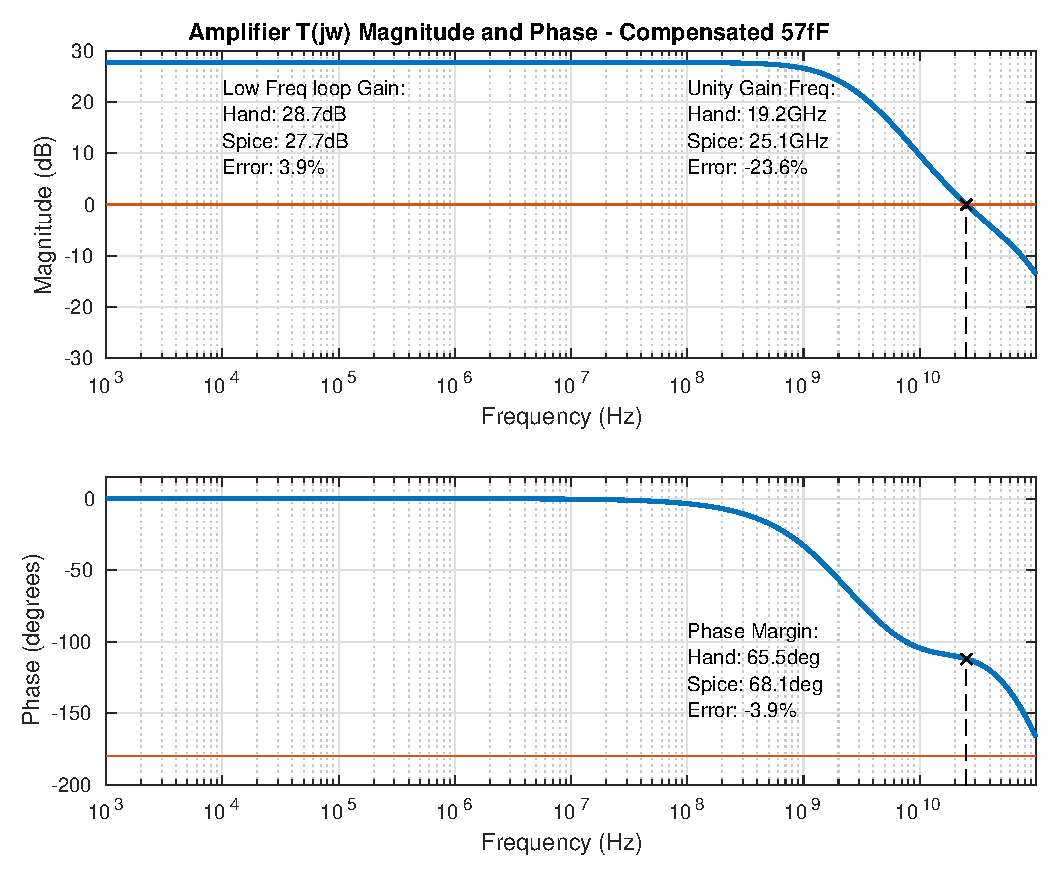
\includegraphics[width=0.8\textwidth]{plots/part_j_t.eps}
\par}

\pagebreak

{\centering
	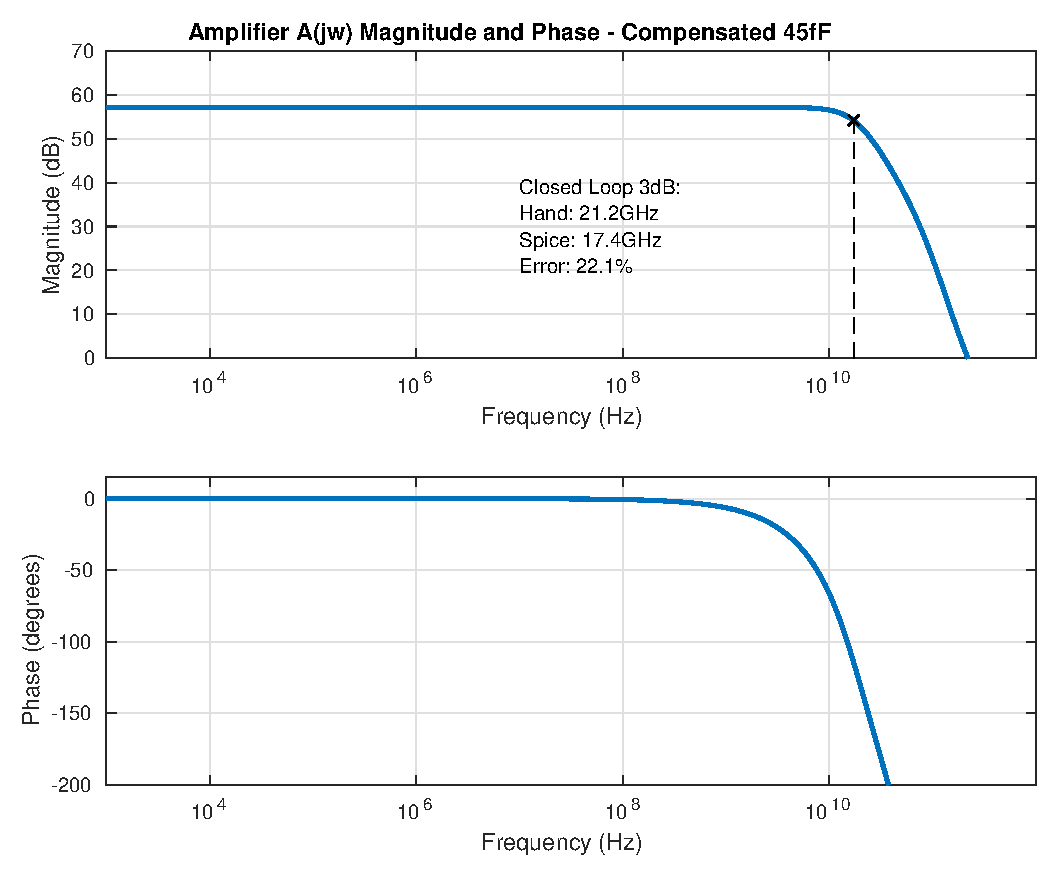
\includegraphics[width=0.8\textwidth]{plots/part_j_a.eps}
\par}

\begin{verbatim}
 ***************************************************
    ******   pole/zero analysis


    input =  0:is          output = v(vo)

    poles (rad/sec)                 poles ( hertz)
    real            imag            real            imag
    -33.1562m       0.              -5.27698m       0.
    -102.336g       -49.5561g       -16.2872g       -7.88710g
    -102.336g       49.5561g        -16.2872g       7.88710g
    -321.575g       358.533g        -51.1803g       57.0622g
    -321.575g       -358.533g       -51.1803g       -57.0622g
    -1.11894t       0.              -178.085g       0.
    -1.35128t       0.              -215.063g       0.
    -1.88412t       0.              -299.868g       0.

    zeros (rad/sec)                 zeros ( hertz)
    real            imag            real            imag
    0.              0.              0.              0.
    -1.09418t       0.              -174.144g       0.
\end{verbatim}

\pagebreak

%%%%%%%%%%%%%%%%%%%%%%%%%%%%%%%%%%%%%%%%%%%%%%%%%%%%%%%%%%%%%%%%%%%%%%%%%%%%%%%%
% Noise - Page 12

% Calculations and simulation plot (with proper annotation) for parts I (k)
% and (l).

\pagebreak

%%%%%%%%%%%%%%%%%%%%%%%%%%%%%%%%%%%%%%%%%%%%%%%%%%%%%%%%%%%%%%%%%%%%%%%%%%%%%%%%
% Transient Rresponse - Page 13

\section{Transient Response - Part I(m)}

{\centering
	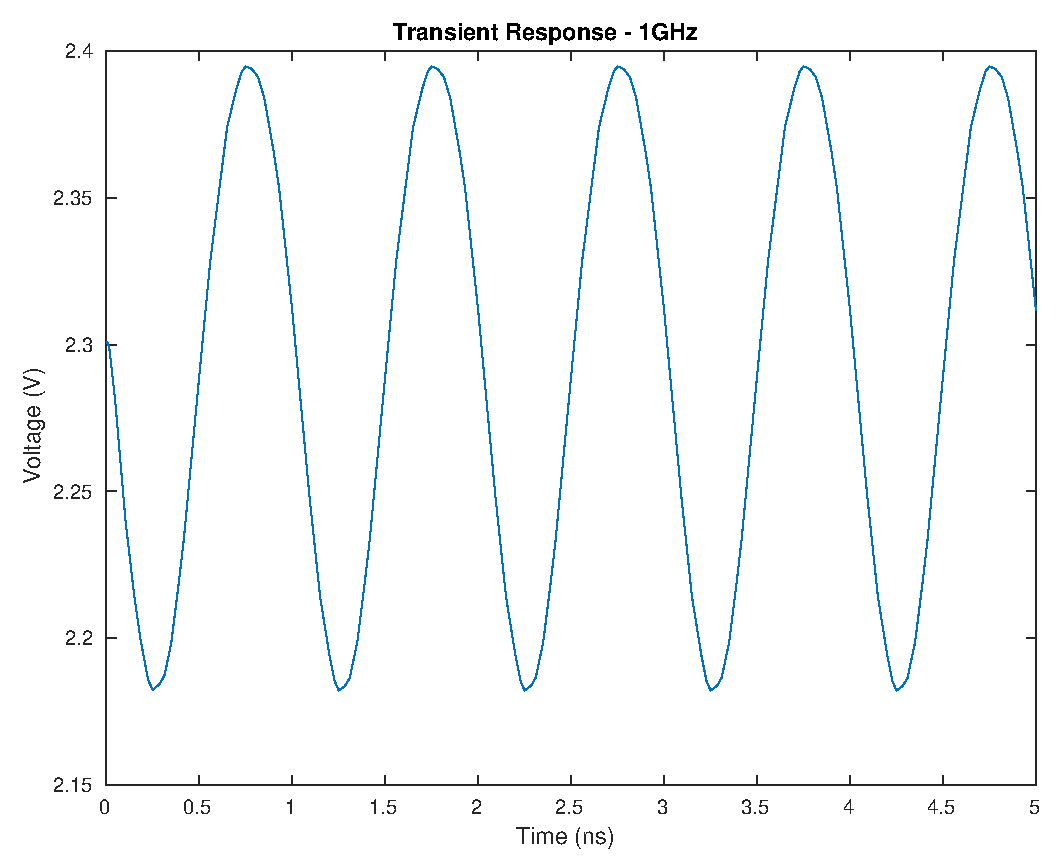
\includegraphics[width=0.8\textwidth]{plots/part_m.eps}
\par}

\pagebreak

\end{document}
